

	





\begin{lstlisting}[language=python]

class Perceptron(object):
"""Perceptron classifier.
Parameters
------------
eta : float
Learning rate (between 0.0 and 1.0)
n_iter : int
Passes over the training dataset.
random_state : int # Random number generator seed for random weight initialization.

Attributes
-----------
w_ : 1d-array
Weights after fitting.
errors_ : list
Number of misclassifications (updates) in each epoch.
"""
def __init__(self, eta=0.01, n_iter=50, random_state=1):
self.eta = eta
self.n_iter = n_iter
self.random_state = random_state

"""Fit training data.
Parameters
----------
X : {array-like}, shape = [n_samples, n_features]
Training vectors, where n_samples is the number of samples and
n_features is the number of features.
y : array-like, shape = [n_samples]
Target values.
Returns
-------
self : object
"""

def fit(self, X, y):

rgen = np.random.RandomState(self.random_state)
self.w_ = rgen.normal(loc=0.0, scale=0.01, size=1 + X.shape[1])
self.errors_ = []

for _ in range(self.n_iter):
errors = 0
for xi, target in zip(X, y):
update = self.eta * (target - self.predict(xi))
self.w_[1:] += update * xi
self.w_[0] += update
errors += int(update != 0.0)
self.errors_.append(errors)
return self

def net_input(self, X): """Calculate net input"""
return np.dot(X, self.w_[1:]) + self.w_[0]

def predict(self, X): """Return class label after unit step"""
return np.where(self.net_input(X) >= 0.0, 1, -1)
\end{lstlisting}


%########################################################################
% CHAP 1
%########################################################################


\subsubsection{\textbf{Développement limité}}\label{sec:dev_lim}
En physique et en mathématiques, un développement limité (noté DL) d'une fonction en un point est une \textit{approximation polynomiale} de cette fonction au voisinage de ce point, c'est-à-dire l'écriture de cette fonction sous la forme de la somme d'une fonction polynomiale et d'un reste négligeable au voisinage du point considéré \cite{coulombeau2013math, benner2015numerical}.

Soit $f$ une fonction à valeurs réelles définie sur un intervalle $I$, et $x_0 \in I$. On dit que $f$ admet un développement limité d'ordre $n^2$ (abrégé par $DL_n$) en $x_0$, s'il existe $n + 1$ réels $a_0, a_1, \dots, a_n$  tels que la fonction ${\displaystyle R:I\to \mathbb {R} }$ définie par :
$${\displaystyle f(x)=a_{0}+a_{1}(x-x_{0})+a_{2}(x-x_{0})^{2}+\dots+a_{n}(x-x_{0})^{n}+R(x)=\sum _{i=0}^{n}a_{i}(x-x_{0})^{i}+R(x)}$$
vérifie : $R(x)$ tend vers $0$ lorsque $x$ tend vers $x_0$, et ce plus rapidement que le dernier terme de la somme, c'est-à-dire que :
$$
\lim _{{x\rightarrow x_{0}}}{\frac{R(x)}{(x-x_{0})^{n}}}=0. 
$$

La fonction reste $R(x)$ vérifiant ceci est notée $o((x – x0)^n)$ (selon la notation de Landau). On écrit donc :

$$
f(x)= \sum _{i=0}^{n}a_{i}(x-x_{0})^{i}+R(x) =\sum _{{i=0}}^{n}a_{i}(x-x_{0})^{i}+o((x-x_{0})^{n})
$$

%\begin{tabular}{r l}
%\( f(x)\) & \( =\sum _{i=0}^{n}a_{i}(x-x_{0})^{i}+R(x)\) \\
%& \(=\sum _{{i=0}}^{n}a_{i}(x-x_{0})^{i}+o((x-x_{0})^{n}) \)
%\end{tabular}

Il est fréquent d'écrire un développement limité en posant $x = x_0 + h$ on aura:

\begin{equation}\label{eq:dev_lim_h}
f(x_{0}+h)=\sum _{{i=0}}^{n}a_{i}h^{i}+o(h^{n})
\end{equation}


\paragraph*{Conséquences immédiates}
\begin{itemize}
	\item Si $f$ admet un $DL_0$ en $x_0$, alors $a_0 = f(x_0)$. \cite{coulombeau2013math}
	\item Si $f$ admet un $DL_n$ en $x_0$, alors elle admet un $DL_k$ en $x_0$ pour tout entier $k < n$ \cite{coulombeau2013math}.
	\item Une condition nécessaire et suffisante pour que f admette un $DL_n$ en $x_0$ est l'existence d'un polynôme $P$ tel que $f(x) = P(x) + o((x – x_0)^n)$ \cite{coulombeau2013math}. S'il existe un tel polynôme $P$, alors il en existe une infinité d'autres, mais un seul d'entre eux est de degré inférieur ou égal à $n$ : le reste de la division euclidienne de $P(X)$ par $(X – x_0)^{n+1}$. On l'appelle la partie régulière, ou partie principale, du $DL_n$ de $f$ en $x_0$. %On identifie parfois, par abus de langage, le $DL_n$ avec sa partie régulière.
\end{itemize}



Le théorème de Taylor-Young assure \cite{coulombeau2013math} qu'une fonction $f$ dérivable $n$ fois au point $x_0$ (avec ${\displaystyle n\geq 1}$ admet un $DL_n$ en ce point :

$$
{\displaystyle f(x)=f(x_{0})+f'(x_{0})(x-x_{0})+{\frac {f''(x_{0})}{2!}}(x-x_{0})^{2}+\dots +{\frac {f^{(n)}(x_{0})}{n!}}(x-x_{0})^{n}+o((x-x_{0})^{n})}
$$

soit en écriture abrégée
$$
f(x)=\sum _{{i=0}}^{n}{\frac  {f^{{(i)}}(x_{0})}{i!}}(x-x_{0})^{i}+o((x-x_{0})^{n})
$$

Le développement d'ordre $0$ en $x_0$ revient à écrire que $f$ est continue en $x_0$ :

$$
{\displaystyle f(x)=f(x_{0})+o((x-x_{0})^{0})=f(x_{0})+o(1)}
$$

Le développement limité d'ordre $1$  en $x_0$ revient à approcher une courbe par sa tangente en $x_0$ on parle aussi d'approximation affine :

\begin{equation}\label{eq:dev_lim_cont}
f(x)=f(x_{0})+f'(x_{0})\cdot (x-x_{0})+o(x-x_{0})
\end{equation}


%\subsubsection{Différentiabilité au sens de Fréchet} \label{sec:drv_frechet}
%Soient $E$ un espace vectoriel normé, $F$ un espace vectoriel topologique séparé, $f$ une application de $E$ dans $F$ et $a$ un point de $E$. On abandonne la notation des vecteurs par des flèches dans ce paragraphe.

%On dit que $f$ est différentiable en $a$ (au sens de Fréchet) s'il existe une application linéaire continue ${\displaystyle L:E\to f}$ telle que :
%$$
%	\forall h\in E\quad f(a+h)=f(a)+L(h)+o\left(\|h\|\right)
%$$
%ou, de manière équivalente :

%$$
%	\lim _{h\to 0}{\frac {f(a+h)-f(a)-L(h)}{\|h\|}}=0.
%$$

%Une telle application linéaire $L$ est alors unique.
%L’opérateur $L$ est appelé différentielle de Fréchet (ou F-différentielle, ou Fréchet-différentielle) de $f$ au point $a$, et $f$ est dite Fréchet-différentiable (ou différentiable, ou différentiable au sens de Fréchet) au point $a$. La différentielle de $f$ au point $a$ est souvent notée $Df(a)$, la notation
%$f'(a)$ est aussi utilisée.
%\subsubsection{Fonctions dérivables}







\subsubsection{\textbf{Hessienne}}
\paragraph*{Définition mathématique:}
Étant donnée une fonction ${f}$ à valeurs réelles

$${ f:\mathbb{R}^{n}\to \mathbb {R} ;(x_{1},...,x_{n})\mapsto f(x_{1},...,x_{n})}$$
dont toutes les dérivées partielles secondes existent, le coefficient d'indice ${ i,j}$ de la \textbf{matrice hessienne\footnote{En mathématiques, la matrice hessienne (ou simplement la hessienne) d'une fonction numérique $f$ est la matrice carrée, notée $H(f)$, de ses dérivées partielles secondes.}} ${H(f)}$ vaut ${H_{ij}(f)={\frac {\partial ^{2}f}{\partial x_{i}\partial x_{j}}}}$ \cite{jtshiman:2021}.\\
Autrement dit,
$$
{ H(f)={
		\begin{bmatrix}{
			\frac {\partial ^{2}f}{{\partial x_{1}}^{2}}}&{\frac {\partial ^{2}f}{\partial x_{1}\partial x_{2}}}&\cdots &{\frac {\partial ^{2}f}{\partial x_{1}\partial x_{n}}}\\
		{\frac {\partial ^{2}f}{\partial x_{2}\partial x_{1}}}&{\frac {\partial ^{2}f}{{\partial x_{2}}^{2}}}&\cdots &{\frac {\partial ^{2}f}{\partial x_{2}\partial x_{n}}}\\
		\vdots &\vdots &\ddots &\vdots \\
		{\frac {\partial ^{2}f}{\partial x_{n}\partial x_{1}}}&{\frac {\partial ^{2}f}{\partial x_{n}\partial x_{2}}}&\cdots &{\frac {\partial ^{2}f}{{\partial x_{n}}^{2}}}
		\end{bmatrix}}} .
$$

\paragraph*{Définition numérique:}
Supposons que $f : \mathbb{R}^{n} \to \mathbb{R}$ définie sur un ouvert $\mathcal{O} \in \mathbb{R}^{n}$. La fonction $f(x)$ est dite 2
fois continûment dérivable (au sens de Fréchet) si en tout $x \in \mathcal{O}$ on a

\begin{equation}
f(x + h) = f(x)+\nabla f(x)^Th + \frac{1}{2}h^T\nabla^2f(x)h+o(||h||^2)
\end{equation}
avec$\nabla f(x)\in \mathbb{R}^{n\times n}$ et où on a posé que le reste 
$ o(||h||^2) =||h|| \epsilon(h) \in \mathbb{R} $ avec 
$\lim\limits_{||h|| \to 0} \epsilon(h) = 0 $
La matrice carrée symétrique $\nabla^2 f(x)$ appelée \textbf{Hessien} de $f(x)$ en $x$ \cite{bierlaire2006introduction}. Remarque :

$$
\lim\limits_{||h|| \to h} \frac{o(||h||^2)}{||h||} = 0  \in \mathbb{R}
$$
La Hessienne s’adresse aux fonctions scalaires à variables vectorielles.
%---------------------------------------------------
%	JACOBIENNE
%---------------------------------------------------		

\subsubsection{\textbf{Jacobienne}}
\paragraph*{Définition mathématique:}
Soit F une fonction d'un ouvert de $\mathbb{R}^{n}$ à valeurs dans $\mathbb{R}^{m}$ ($F:\mathbb{R}^{n}\to \mathbb {R}^{m}$). Une telle fonction est définie par ses $m$ fonctions composantes à valeurs réelles :

$$ 
{ F:
	{\begin{pmatrix}
		x_{1}\\\vdots \\
		x_{n}
		\end{pmatrix}}
	\longmapsto 
	{\begin{pmatrix}
		f_{1}(x_{1},\dots ,x_{n})\\
		\vdots \\f_{m}(x_{1},\dots ,x_{n})
		\end{pmatrix}}}.
$$
Les dérivées partielles de ces fonctions en un point $M$, si elles existent, peuvent être rangées dans une matrice à $m$ lignes et $n$ colonnes \cite{jtshiman:2021}, appelée \textbf{matrice jacobienne\footnote{En analyse vectorielle, la matrice jacobienne est la matrice des dérivées partielles du premier ordre d'une fonction vectorielle en un point donné.}} de $F$ :
$$
J_{F}\left(M\right)={
	\begin{pmatrix}
	{\dfrac {\partial f_{1}}{\partial x_{1}}}&\cdots &{\dfrac {\partial f_{1}}{\partial x_{n}}}\\
	\vdots &\ddots &\vdots \\
	{\dfrac {\partial f_{m}}{\partial x_{1}}}&\cdots &{\dfrac {\partial f_{m}}{\partial x_{n}}}
	\end{pmatrix}}.
$$

La case sur la ligne $i$ et la colonne $j$ contient ${\displaystyle {\frac {\partial f_{i}}{\partial x_{j}}}}$ qui est la dérivée partielle de $f_i$ selon la variable $x_j$. Cette matrice est notée :

$${\displaystyle J_{F}\left(M\right),\qquad {\frac {\partial \left(f_{1},\ldots ,f_{m}\right)}{\partial \left(x_{1},\ldots ,x_{n}\right)}}\qquad {\text{ou}}\qquad {\frac {\mathrm {D} \left(f_{1},\ldots ,f_{m}\right)}{\mathrm {D} \left(x_{1},\ldots ,x_{n}\right)}}}$$

Pour $i = 1, … , m,$ la i-ème ligne de cette matrice est la transposée du vecteur \textbf{gradient} (voir le point \ref{sec:gradient}) au point $M$ de la fonction $f_i$, lorsque celui-ci existe. La matrice jacobienne est également la matrice de la différentielle de la fonction, lorsque celle-ci existe \cite{jtshiman:2021}.
\paragraph*{Définition numérique:}

Soit $f(x) : \mathbb{R}^n \to \mathbb{R}^m$ définie sur un ouvert $ \mathcal{O} \subset \mathbb{R} $. On dit que $f(x)$ est dérivable
(au sens de Fréchet) en $x$, si chacune des composantes $f_i(x)$ est dérivable  en $x$ \cite{bierlaire2006introduction}. On a alors

\begin{equation}
f(x + h) = f(x) + D_f (x)h + o(||h||)
\end{equation}
avec $D_f (x) \in  \mathbb{R}^{n \times m} $ et/où $ o(||h||)=||h|| \epsilon(h) \in \mathbb{R}^m $ avec $\lim\limits_{||h|| \to 0} \epsilon(h) = 0 $.
Remarque :
$$
\lim\limits_{||h|| \to h} \frac{o(||h||^2)}{||h||} = 0  \in \mathbb{R}
$$

Soient 
$x = 
\begin{bmatrix}
x_1 & x_2& \cdots & x_n
\end{bmatrix}^{T}
\in \mathbb{R}^n $ et $ 
f(x) = 
\begin{bmatrix}
f_1(x) & f_2(x)& \cdots & f_n(x)
\end{bmatrix}^{T} \in \mathbb{R}^m
$

$$
D_f\left(x\right)={
	\begin{bmatrix}
	{\dfrac {\partial f_{1}(x)}{\partial x_{1}}}&\cdots &{\dfrac {\partial f_{1}(x)}{\partial x_{n}}}\\
	\vdots &\ddots &\vdots \\
	{\dfrac {\partial f_{m}(x)}{\partial x_{1}}}&\cdots &{\dfrac {\partial f_{m}(x)}{\partial x_{n}}}
	\end{bmatrix}}
=
\begin{bmatrix}
\nabla f_1(x)^T \\ \nabla f_2(x)^T\\ \vdots \\ \nabla f_m(x)^T
\end{bmatrix}
\in  \mathbb{R}^{n \times m},
$$
La matrice $D_f (x) \in  \mathbb{R}^{n \times m} $ est appelée \textbf{Jacobienne} de f(x) en x.
La Jacobienne s’adresse aux fonctions vectorielles à variables vectorielles \cite{jtshiman:2021}.

\begin{description}
	\item[Note:] Lorsque $m=1$ (m : nombre des lignes), la Jacobienne est la même que le gradient car il s'agit d'une généralisation du gradient.
\end{description}





		

\subsection{Échantillonnage (statistique)} \label{sec:chantillonnage} % \& probabilité bayésienne}

%\subsubsection{Échantillonnage (statistique)}

En statistiques, l'échantillonnage est la sélection d'un sous-ensemble (un échantillon statistique ) d'individus au sein d'une population statistique pour estimer les caractéristiques de l'ensemble de la population. \\
Sur un échantillon, on peut calculer différents paramètres statistiques de position ou de dispersion issus de la statistique descriptive, de la même manière que l'on peut déterminer des paramètres statistiques d'une population par son recensement exhaustif \cite{sarndal2003model}.

On peut également déduire des propriétés de la population à partir de celles de l'échantillon par inférence statistique. D'après la loi des grands nombres, plus la taille de l'échantillon augmente, plus ses propriétés seront proches de celles de la population. En particulier, on peut estimer une probabilité sur les individus d'une population par la fréquence observée sur un échantillon si sa taille est suffisamment grande \cite{sarndal2003model, harrell2001regression}. 

Cette méthode présente plusieurs avantages : une étude restreinte sur une partie de la population, un moindre coût, une collecte des données plus rapide que si l'étude avait été réalisée sur l'ensemble de la population, la réalisation de contrôles destructifs, etc.
Un dataset assez large permettra ainsi  à une machine d'effectuer un bon apprentissage automatique sur cet ensemble de données constituant l'échantillon de la population a apprendre.

\begin{list}{$\triangleright$ }{On peut procéder de différentes manières pour collecter les données de l'échantillon, il existe en effet plusieurs méthodes d'échantillonnage \cite{sarndal2003model} :}
	%\textbf
	\item  \textbf{Échantillonnage aléatoire et simple }: le tirage des individus de l'échantillon est aléatoire, c'est-à-dire que chaque individu a la même probabilité d'être choisi, et simple, c'est-à-dire que les choix des différents individus sont réalisés indépendamment les uns des autres.
	%L'échantillonnage aléatoire simple peut être vulnérable aux erreurs d'échantillonnage car le caractère aléatoire de la sélection peut donner un échantillon qui ne reflète pas la composition de la population. 
	
	\item  \textbf{Échantillonnage systématique }: le premier individu est choisi de manière aléatoire, puis les suivants sont déterminés à intervalle régulier. Par exemple, dans un verger, on choisit au hasard le 7e pommier, puis les 27e, 47e, 67e, etc.
	
	\item  \textbf{Échantillonnage stratifié }: on subdivise la population en plusieurs parties avant de prendre l'échantillon1.
	
	\item \textbf{Échantillonnage par quotas }: la composition de l'échantillon doit être représentative de celle de la population selon certains critères jugés particulièrement importants. On utilise cette méthode pour réaliser les sondages d'opinions.
\end{list}


\subsubsection{\textbf{La collecte de données} }

La collecte de données est le processus de collecte et de mesure des informations sur des variables ciblées dans un système établi, qui permet ensuite de répondre aux questions pertinentes et d'évaluer les résultats.

\begin{list}{--}{Une bonne collecte de données implique :}
	\item Suivre le processus d'échantillonnage défini
	\item Garder les données dans l'ordre du temps
	\item Noter les commentaires et autres événements contextuels
	\item Enregistrement des non-réponses
\end{list}

\paragraph*{Erreur d'échantillonnage :}
Dans les statistiques, les erreurs d'échantillonnage se produisent lorsque les caractéristiques statistiques d'une population sont estimées à partir d'un sous-ensemble, ou échantillon, de cette population. Étant donné que l'échantillon n'inclut pas tous les membres de la population, les statistiques de l'échantillon (souvent appelées estimateurs), telles que les moyennes et les quartiles, diffèrent généralement des statistiques de l'ensemble de la population (appelées paramètres ). La différence entre la statistique d'échantillon et le paramètre de population est considérée comme l'erreur d'échantillonnage \cite{sarndal2003model}. 




%\subsubsection{Généralité sur l'analyse bayésienne}
%La statistique bayésienne est une théorie dans le domaine des statistiques basée sur l' interprétation bayésienne de la probabilité où la probabilité exprime un degré de croyance en un événement. Le degré de croyance peut être basé sur des connaissances antérieures sur l'événement, telles que les résultats d'expériences précédentes, ou sur des croyances personnelles sur l'événement. Cela diffère d'un certain nombre d'autres interprétations de la probabilité , telles que l' interprétation fréquentiste qui considère la probabilité comme la limite de la fréquence relative d'un événement après de nombreux essais [??].

%Les statistiques bayésiennes portent le nom de Thomas Bayes qui a formulé un cas spécifique du théorème de Bayes dans un article publié en 1763.



%\begin{thm}[Théorème de Bayes] Le théorème de Bayes est utilisé dans les méthodes bayésiennes pour mettre à jour les probabilités, qui sont des degrés de croyance, après avoir obtenu de nouvelles données. Compte tenu de deux événements $A$  et $B$, la probabilité conditionnelle de $A$ étant donné que $B$ est vrai s'exprime comme suit  :
%\begin{equation}
%\mathbb{P}(A|B) = \frac{\mathbb{P}(B|A) \mathbb{P}(A)}{\mathbb{P}(B)}
%\end{equation}

%\end{thm}

%où $\mathbb{P}(B) \ne 0$ Bien que le théorème de Bayes soit un résultat fondamental de la théorie des probabilités , il a une interprétation spécifique dans les statistiques bayésiennes \cite[][]{antoine2018apprentissage}.

%%%%%%%%%%%%%%%%%%%%%%%%%%%%%%%%%%%%%%%%%%%%%%%%%%%%%%%%%%%%%%%%%%%%%%%%%%%%%%%%%%%%%
% SECTION 2
%%%%%%%%%%%%%%%%%%%%%%%%%%%%%%%%%%%%%%%%%%%%%%%%%%%%%%%%%%%%%%%%%%%%%%%%%%%%%%%%%%%%%

\subsubsection{\textbf{Les ingrédients d'apprentissage}}
Résoudre un problème d'apprentissage, c'est d'abord le comprendre, c'est-à-dire discuter longuement avec les experts, ou consulter les ouvrages, du domaine concerné pour identifier quelles sont les "entrées", les  "sorties" ou résultats désirés, les connaissances disponibles, les particularités des données, par exemple: valeurs manquantes, taux de bruit dans les mesures des attributs de description, proportions des classes, stationnarité ou pas de l'environnement.\\ 
C'est aussi réaliser un gros travail de \textit{préparation des données}: nettoyage, ré-organisation, enrichissement, intégration avec d'autres sources de données, etc. Ces étapes de compréhension du problème, de préparation des données, de mise au point du protocole d'apprentissage et des mesures d'évaluation des résultats, prennent, et de loin, la plus grande partie du temps pour (tenter de) résoudre un problème d'apprentissage \cite{antoine2018apprentissage}. 
Nous avons toujours tendance à largement sous-estimer ces étapes et à vouloir se concentrer uniquement sur la phase excitante de l'essai de méthodes d'apprentissage sur des données supposées bonnes à la consommation \cite{darlington2016regression}. 
%\subsubsection{Algorithme qui apprennent}



	La table suivante présente d'abord les qualités des différentes représentations des hypothèses en fonction des critères cités ci-dessus.


%\parbox[t]{2mm}{\multirow{3}{*}{\rotatebox[origin=c]{90}{rota}}} 
\begin{center}
	\begin{tabular}{l|cccccc}
		& \rotatebox[origin=c]{90}{Fonctions séparatrices}
		&  \rotatebox[origin=c]{90}{Distributions de probabilités}
		& \rotatebox[origin=c]{90}{Arbres de décision }
		& \rotatebox[origin=c]{90}{Hiérarchies de concepts}
		& \rotatebox[origin=c]{90}{Réseaux bayésiens } 
		& \rotatebox[origin=c]{90}{Chaînes de Markov}\\
		\hline
		
		Concept & $\surd$ &$\surd$ &$\surd$ &$\surd$ & --&-- \\
		Classes multiples &$\surd$ & $\surd$ &$\surd$ &$\surd$ &--&-- \\
		Ontologies & --&-- & $\surd$&$\surd$ & --&-- \\
		Régression &-- &$\surd$ & $\surd$&-- &-- &-- \\
		Évolutions temporelles &-- &$\surd$ &-- &-- &-- & $\surd$\\
		Apprentissage non supervisé & $\surd$ &$\surd$ &$\surd$ &$\surd$ &-- &-- \\
		Données continues & $\surd$ &$\surd$ &$\surd$ &-- &-- &$\surd$  \\
		Connaissances relationnelles  & & & & $\surd$  & $\surd$  &-- \\
		Degré de certitude &-- &$\surd$ &-- &-- &$\surd$ &$\surd$ \\
		Degré d'imprécision &-- &$\surd$ &-- &-- &$\surd$ &-- \\
		Transparence, intelligibilité &-- &-- &-- &$\surd$ &$\surd$ &$\surd$ \\
		%& & & & \\
		%& & & & \\
		
		
	\end{tabular}
\end{center}



\subsubsection{Le cas de la régression linéaire}
On appelle problèmes de régression de tels problèmes, dans lesquels la sortie est numérique, généralement un vecteur de réels, supposé dépendre de la valeur d'un certain nombre de facteurs en entrée \cite{matloff2017statistical,darlington2016regression}.

\begin{figure}[hth]%bth
	\centering
	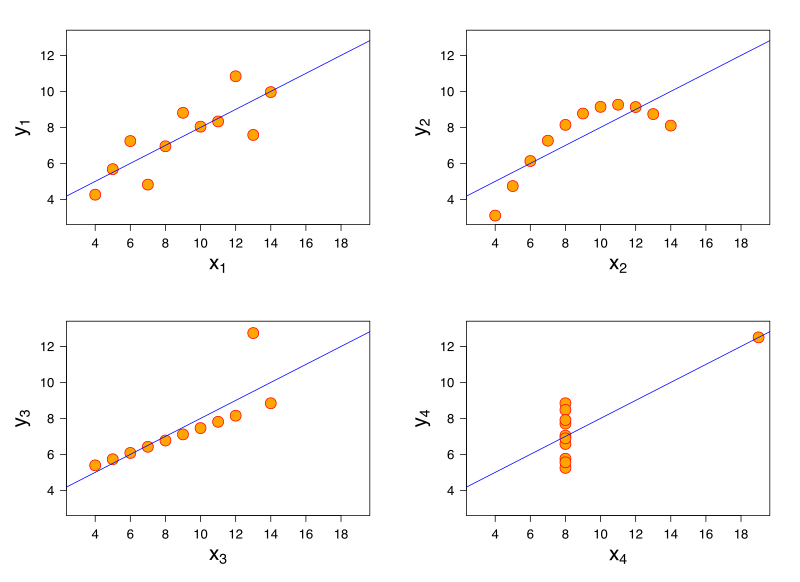
\includegraphics[width=\textwidth]{images/linear_regression_quartet.png}
	\caption{Images illustrant l'efficacité de la régression linéaire sur plusieurs type de modèle.}
	\label{fig:linear_regression_quartet}
\end{figure}

Le vecteur d'entrée $x = (x_1,x_2,...,x_n)^T$ est souvent appelé variable indépendante, tandis que le vecteur de sortie $y$ est appelé variable dépendante. On formalise le problème en supposant que la sortie résulte de la somme d'une fonction déterministe $f$ de l'entrée et d'un bruit aléatoire :
\begin{equation}
y = f(x) + \epsilon
\end{equation}

où $f(x)$ est la fonction inconnue que nous souhaitons approcher par un estimateur $h(x|w)$, où $h$ est défini à l'aide d'un vecteur $w$ de paramètres \cite{alpaydin2010introduction}.
Si l'on suppose que le bruit $\epsilon$ est nulle et de variance constante $\sigma^2$, c'est-à-dire $ \epsilon = \mathcal{N}(0,\sigma^2)$, alors, en plaçant notre estimateur $h(\cdot)$ à la place de la fonction inconnue, on devrait avoir la densité conditionnelle réelle $p(y|x)$ vérifiant :
\begin{equation}
p(y|x) = \mathcal{N}(h(x|w),\sigma^2)
\end{equation}

On peut estimer le vecteur de paramètres $w$ grâce au principe de maximisation de la vraisemblance. On suppose que les couples $(x_t, y_t)$ de l'échantillon d'apprentissage sont tirés par tirages indépendants d'une distribution de probabilités jointes inconnue $p(x, y)$, qui peut s'écrire :

$$
p(y|x) = p(y|x)p(x)
$$
où $p(y|x)$ est la probabilité de la sortie étant donnée l'entrée et $p(x)$ est la densité de probabilité sur les entrées \cite{matloff2017statistical}.

%Étant donné un échantillon d'apprentissage $S = \langle (x_t,y_t) \rangle_{1\leq t\leq m} $ supposé tiré de manière indépendante et identiquement distribuée.
%Maximiser l'expression résultante revient alors à minimiser la somme de carrés des erreurs (SCE) \cite{antoine2018apprentissage}:
%\begin{equation}\label{eq:sce_1}
%SCE(w|\mathit{S}) = \frac{1}{2} \sum_{{t=1}}^{m}{ [ y_t - h(x_t|w) ]^2}	
%\end{equation}

%%%\subsubsection*{La régression non linéaire ou multiple}



	\subsubsection{Calcul avec l'algorithme du perceptron}

Le premier concept de règle d'apprentissage du perceptron, a été publié par Frank Rosenblatt \cite{antoine2018apprentissage}, basé sur le modèle neuronal MP Neuron (McCulloch-Pitts Neuron). 

%(F. Rosenblatt, The Perceptron, a Perceiving and Recognizing Automaton. Cornell Aeronautical Laboratory, 1957).

Avec sa règle de perceptron, Il a proposé un algorithme qui apprendrait automatiquement les coefficients de poids optimaux qui sont ensuite multipliés par les caractéristiques d'entrée afin de décider si un neurone se déclenche ou non. Dans le cadre de l'apprentissage supervisé et de la classification, un tel algorithme pourrait alors être utilisé pour prédire si un échantillon appartient à une classe ou à l'autre \cite{ml2008python}.

Il est important de noter que la convergence du perceptron n'est garantie que si les deux classes sont linéairement séparables et que le taux d'apprentissage %footenot : taux d'apprentissage definition 
est suffisamment faible. Si les deux classes ne peuvent pas être séparées par une limite de décision linéaire, nous pouvons définir un nombre maximum de passages sur l'ensemble de données d'apprentissage (époques) et/ou un seuil pour le nombre d'erreurs de classification tolérées - le perceptron n'arrêterait jamais de mettre à jour les poids autrement \cite{freund1999large, ml2008python}.

L'algorithme du perceptron travaille directement sur le vecteur a qui caractérise la surface discriminante cherchée. On n'a donc plus besoin ici de se placer dans l'espace de représentation de dimension n+1. Cet algorithme utilise un protocole d'apprentissage itératif : il prend les données d'apprentissage les unes après les autres, chacune étant choisie soit par un passage systématique dans l'ensemble d'apprentissage (version \textit{« non stochastique »}), soit par un tirage au hasard dans celui-ci (version\textit{ « stochastique »}). Son nombre d'étapes effectives peut être important: un seul (exactement ou en moyenne) passage des données n'est en effet pas suffisant pour le faire converger (voir le chapitre \ref{chap:methode}, section \ref{sec:convergence_sgd}). \cite{antoine2018apprentissage}.

%\begin{algorithm}[H]
%	\caption{Perceptron, version stochastique}
%	\begin{algorithmic} 
%		\REQUIRE $n \geq 0 \vee x \neq 0$
%		\STATE $t \leftarrow 0$		
%		\WHILE{$N \neq 0$}
%			\STATE get random $x_i \in X$ set
%			\IF{$x$ is classed}
%				\STATE $a_{t+1} \leftarrow a_t$
%			\ELSE[]
%				\IF{$x \in \mathcal{W}_1$}
%					\STATE	$a_{t+1} \leftarrow a_t + \alpha x$
%				\ELSE[]
%					\STATE	$a_{t+1} \leftarrow a_t - \alpha x$
%				\ENDIF
%				\STATE $t \leftarrow t + 1 $
%			\ENDIF
%		\ENDWHILE		
%	\end{algorithmic}
%\end{algorithm}


\begin{lstlisting}[language=python]
class Perceptron(object):
# Parametres
eta : float # taux d'apprentissage (between 0.0 and 1.0)
n_iter : int # nombre d'iteration
random_state : int # generateur de nombres aleatoires pour l'initialisation de poids aleatoire.
w_ : list # Poids apres fitting.
errors_ : list # Nombre d'erreurs de classification (mises a jour) a chaque epoque.

def __init__(self, eta=0.01, n_iter=50, random_state=1):
self.eta = eta
self.n_iter = n_iter
self.random_state = random_state

# Parameters
X : list, # matrice d'echantillons de taille = (n \times m).
y : list, # vecteur de taille = n, qui contient les valeurs cibles.

def fit(self, X, y): # Ajuster les donnees d'entrainement (Fit training data).
rgen = np.random.RandomState(self.random_state)
self.w_ = rgen.normal(loc=0.0, scale=0.01, size=1 + X.shape[1])
self.errors_ = []

for _ in range(self.n_iter):
errors = 0
for xi, target in zip(X, y):
update = self.eta * (target - self.predict(xi))
self.w_[1:] += update * xi
self.w_[0] += update
errors += int(update != 0.0)
self.errors_.append(errors)
return self

def net_input(self, X): # Calculer la sortie net
return np.dot(X, self.w_[1:]) + self.w_[0]

def predict(self, X):
return np.where(self.net_input(X) >= 0.0, 1, -1)
\end{lstlisting}





%########################################################################
%
%########################################################################









%########################################################################
%
%########################################################################









%########################################################################
%
%########################################################################









%########################################################################
%
%########################################################################